\section{Architecture}
\label{SEC:architecture}

\begin{figure}[t]
  \center{}
  \fbox{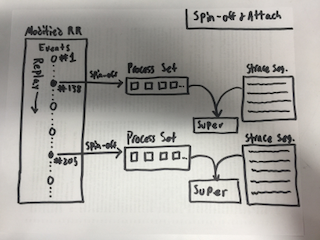
\includegraphics[scale=.75]{architecture}}
  \caption{Diagram illustrating CrashSimulator's Architecture.  During the
    course of a single rr execution, clone process sets are generated at
    specific rr events.  A CrashSimlator supervisor process attaches to
    these process sets and uses a strace-style system call listing to feed
    subsequent system call activity and inject unusual environmental
    conditions.}
  \label{figure:architecture}
\end{figure}

CrashSimulator's testing process
consists of launching the application under test as a child process and
interceeding in its execution at appropriate times in order to simulate the
results and side effects of any system call the application might make.
Implementing CrashSimulator's testing approach requires XX pieces of
functionality:  First, there must be some way to have
repeatable execution of the application under test. This ensures that
the interesting system call sequence is reached.  Second, there must be
some way to interpose on on execution in order modify the results and side
effects of system calls in such a way that they reflect the environmental
anomaly the application is being exposed to.  Our current iteration of
CrashSimulator uses a modified version of {\tt rr} to handle the first
requirement and a custom CrashSimulator process supervisor to handle the
second.

{\tt rr} is an excellent candidate for handling repeatable executions
because of its advanced record-and-replay capabilities.  It is able to
record and replay applications quickly and accurately out right out of the
box which is valuable in both human-in-the-loop and automated
continuous integration/continuous deployment testing scenarios.  Replay
executions occur as a sequence of ``events'' which map to application
events like system calls and signals.  We modified {\tt rr} so that it
could be made to run to a specific event corresponding to specific system
call and generate clones of the set of processes being replayed at that
point in time.  These cloned process sets exist entirely separately from
{\tt rr} allowing it to continue through its replay process to the next
designated event.  This means that one {\tt rr} replay execution can spin
off as many process sets as are required to perform the set of tests
configured by the user.

Process sets generated by {\tt rr} are created in a stopped state and
remain until they are attached to and utilized by a CrashSimulator
supervisor.  Each process set has its own supervisor process which injects
its configured environmental anomaly.  This is accomplished by the
supervisor waking up the process set it is managing and simulating any
subsequent system calls it makes.  The data necessary for this
simulation is
supplied as a system call listing formatted after the style of {\tt strace}
output. This listing describes the results and side effects for each system
call engineered in such a way that the elements required to reflect the
desired environmental anomaly is present.  Supervisors can complete this
process independently of one another lending a high degree of speed and
parallelism to the whole CrashSimulator testing process.

\subsection{Implementation}

We built CrashSimulator to operate on a modern 32-bit Linux kernel running
on Ubuntu 16.04 LTS.  Our modifications to {\tt rr} were carried out in C++
and the CrashSimulator supervisor was implemented in ZZZZ lines of Python
2.7. code with a YYYY line C extension that allows it to interact with
processes using the {\tt Ptrace} API.  This version of CrashSimulator is
available as a Docker container and, due to some operating system
configuration being necessary, is most easily installed in this fashion.
